\documentclass[svgnames,tikz]{standalone}
\usepackage{pgfplots}

\begin{document}

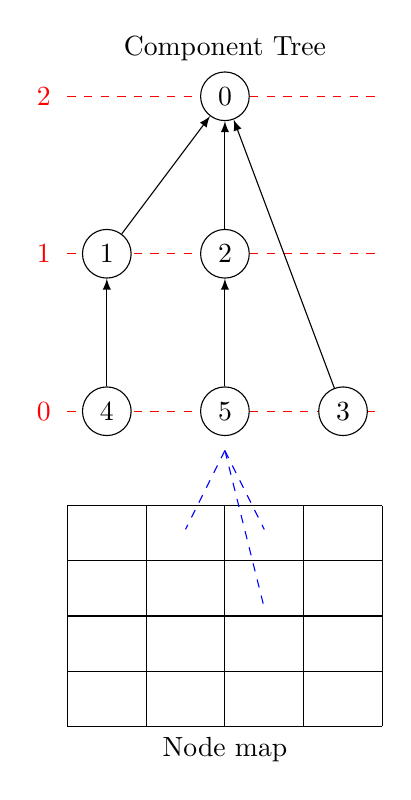
\begin{tikzpicture}
	\draw[y=0.7cm, step=1] (0, 0) grid (4, 4);

	\draw[dashed, red] (0, 4) -- (4, 4);
	\draw[dashed, red] (0, 6) -- (4, 6);
	\draw[dashed, red] (0, 8) -- (4, 8);

	\node[red] () at (-0.3, 4) {0};
	\node[red] () at (-0.3, 6) {1};
	\node[red] () at (-0.3, 8) {2};

	\node[draw, circle, fill=white] (0) at (2, 8) {0};
	\node[draw, circle, fill=white] (1) at (0.5, 6) {1};
	\node[draw, circle, fill=white] (2) at (2, 6) {2};
	\node[draw, circle, fill=white] (3) at (3.5, 4) {3};
	\node[draw, circle, fill=white] (4) at (0.5, 4) {4};
	\node[draw, circle, fill=white] (5) at (2, 4) {5};

	\draw[->, >=latex] (1) -- (0);
	\draw[->, >=latex] (2) -- (0);
	\draw[->, >=latex] (3) -- (0);
	\draw[->, >=latex] (4) -- (1);
	\draw[->, >=latex] (5) -- (2);

	\draw[blue, dashed] (2, 3.5) -- (2.5, 2.5);
	\draw[blue, dashed] (2, 3.5) -- (2.5, 1.5);
	\draw[blue, dashed] (2, 3.5) -- (1.5, 2.5);

	\node () at (2, -0.3) {Node map};
	\node () at (2, 8.6) {Component Tree};

\end{tikzpicture}

\end{document}